\section{About this document}
	\label{sec:AboutThisDocument}

	\change{Note}{25}{The 9/2020 version does not have this appendix and it is included for document management purposes }

	\begin{wrapfigure}{o}{0.3\textwidth}
		\centering
		\vspace{-30pt}
		\fbox{
\includegraphics[width=1.5in]{images/qr_code_github_repo.png}}
		\caption{Document files on Github}
		\label{fig:qr_repo}
		\vspace{10pt}
		\fbox{
\includegraphics[trim=25 25 25 25,clip,width=1.5in]{images/qr_releases.png}}
		\caption{Folder containing handbook pdf files}
		\label{fig:qr_releases}
	\end{wrapfigure}


	This document is an official governing document for Westmont College so changes are carefully managed and subject to a formal approval process
	(See Section
	\ref{sec:ProtocolsForRevision},
	``\nameref{sec:ProtocolsForRevision}''
	) .
	To support the integrity of the document, it is stored in a Github repository which functions as its change management system and supports transparency into any document modifications.
	The original LaTeX source documents can be found in that repository located
	\href{https://github.com/djp3/WestmontFacultyHandbook}{here}.
	(qr code in Figure \ref{fig:qr_repo}).


	\subsection{Current Version}


		To make sure that you have the latest version of this document, compare the version and date in the
		footer of this document with the dates in the footers of the current versions that are online.
		All released versions can be found in
		\href{https://github.com/djp3/WestmontFacultyHandbook/tree/main/releases}{the releases} folder of the Github repository.
		(qr code in Figure \ref{fig:qr_releases}) including:
		\begin{itemize}
			\item{{\bfseries handbook.pending.pdf}:
				The current working document including pending changes, labelled
				. This includes notated changes that have not been formally approved by the Board of Trustees}
			\item{{\bfseries handbook.approved.pdf}:
				The official version that has been approved by the Board of Trustees, labelled ``handbook.approved.pdf''.}
			\item{Historical versions for reference, labelled as such}
		\end{itemize}

	\subsection{Proposing Changes}
		\subsubsection{Technical Mechanism for Changes}
			Using the features of github, it is possible to submit changes
			directly to the source text of this document by editting
			it online. To accomplish this,
			navigate to the website identified in Figure \ref{fig:qr_repo} and
			edit the files that end in ``.tex''

			Such edits will be noted as proposed changes and are called ``pull requests'' by github.
			The changes will need to be voted on by the Faculty Council before the pull request will be accepted, thus changing the document.

			Alternatively, one can open an ``issue'' on the website to propose a change in general terms.  The issue has its own
			comment thread.

			Once the changes are approved via a formal process, the document must be typeset and submitted to the repository for distribution.
		\subsubsection{Techno-social Mechanism for Changes Initiated by Faculty}
			\begin{center}
				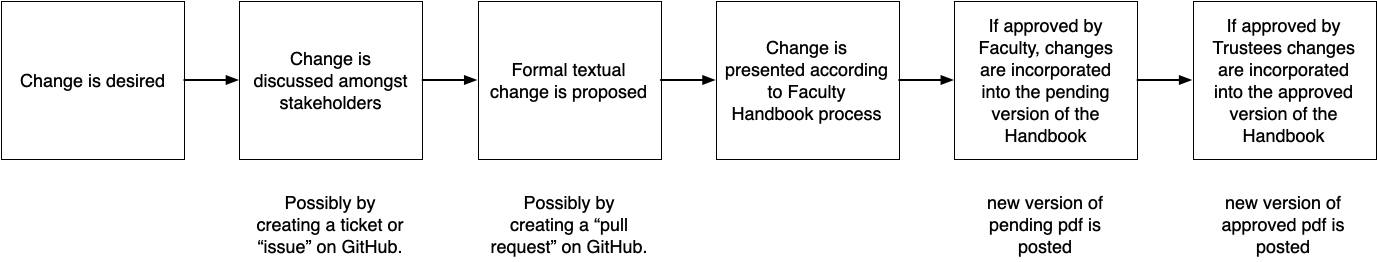
\includegraphics[width=\textwidth]{images/change_process.png}
			\end{center}





